\documentclass[twoside]{article}

\usepackage{todonotes}
\usepackage{hyperref}
\usepackage{fancyhdr}
\usepackage{enumerate}

\pagestyle{fancy}
\rfoot{Document number: RBB4-01}

\graphicspath{{img/}}

\begin{document}
\title{Minor Change}
\author{}
\date{}
\maketitle

\section{Change design description}
Design title: Installation of a transponder and antenna in a Pilatus B4 glider.

\section{Aircraft identification}
\begin{tabular}{|l|l|}
\hline
Aircraft type & Serial Number \\
\hline
Pilatus B4 & All \\
Pilatus B4A & All \\
Pilatus B4AF & All \\
\hline
\end{tabular}

\section{Design summary}
This change is made to install a TSO-approved Mode-S transponder (like for example the Garrecht VT-01 UltraCompact) with a Filser Transflex-4 antenna in the applicable aircraft. The design covers the installation of an antenna, a transponder and wiring. This change is identical for all effective aircraft.

\section{Applicable requirements}
\subsection[CS 22.1301]{CS 22.1301:  Equipment/Function and installation}
\begin{enumerate}[(a)]
\item Each item of required equipment must:
	\begin{enumerate}[(1)]
          \item be of a kind and design appropriate to its intended function;
          \item be labelled as to its identification, function, or operating limitations, or any applicable combination of these factors;
          \item be installed according to limitations specified for that equipment; and
          \item function properly when installed. (See AMC 22.1301(a)(4))
	\end{enumerate}
\item Instruments and other equipment may not in themselves, or by their effect upon the sailplane, constitute a hazard to safe operation.
\end{enumerate}


\subsection[CS 22.1365]{CS 22.1365:  Electrical Systems and Equipment/Electric cables and equipment}
\begin{enumerate}[(a)] 
\item Each electric connecting cable must be of adequate capacity and correctly routed, attached and connected so as to minimize the probability of short circuits and fire hazards.
\item Overload protection must be provided for each electrical equipment. No protective device may protect more than one circuit essential to flight safety.
\item Unless each cable installation from the battery to a circuit protective device or master switch, whichever is closer to the battery, is of such power-carrying capacity that no hazardous damage will occur in the event of a short circuit, this length of cable must be so protected or routed in relation to parts of the powered sailplane that the risk of short circuit is minimised. (See AMC 22.1365(c))
\end{enumerate}

\subsection[CS 22.1431]{CS 22.1431:  Miscellaneous Equipment/ATC airborne equipment}
Each ATC airborne equipment provided must comply with the following:
\begin{enumerate}[(a)]
\item The equipment and its aerials may neither in themselves nor by their mode of operation or by their effect upon the operating characteristics of the sailplane and its equipment constitute a hazard to safe operation.
\item The equipment and its control and monitoring devices must be arranged so as to be easily controllable. Their installation must be such that they are sufficiently ventilated to prevent overheating.
\end{enumerate}


\subsection[EuroCAE ED-73B]{EuroCAE ED-73B: Minimum operational performance specifications for secondary surveillance radar mode s transponders}
These minimum operational performance specifications are designed to ensure that aircraft Mode S Secondary Surveillance Radar (SSR) transponder equipments certificated to them will be compatible with ICAO Annex 10, Volume IV, Part I up to Amendment 82 and the 1st edition of ICAO Document 9871 (Technical Provisions for Mode S Services and Extended Squitter). 

These minimum operational performance specifications do not include detailed descriptions of Mode S coding formats, protocols and interfaces; these can be found in ICAO Annex 10, Volume IV. 

\section{Minor/Major classification}
The change has no appreciable effect on the mass, balance, structural strength, reliability, operational characteristics, noise, fuel venting, exhaust emission, or other characteristics affecting the airworthiness of this product. Therefore, this change can be considered Minor.

\section{Weigth and balance}
After the change has been performed, a new weight \& balance report must be made. This can be performed by either weighing of the aircraft or by calculation.

\section{Substantiation of the requirements}

\subsection[CS 22.1301]{CS 22.1301:  Equipment/Function and installation}
\begin{enumerate}[(a)]
\item For each item the following applies:
\begin{enumerate}[(1)]
\item This Minor Change only covers the installation of ETSO-2C112a approved transponders, such as the Garrecht VT-01 UltraCompact. The antenna Filser Transflex-4 or equivalent will be installed. According to the manufacturer data of the transponder any suitable antenna may be used.
\item Transponders with ETSO-2C112a approval are clearly identifiable as transponders. Use, limitations of its use etc. are to be found in the user manual of the relevant transponders.
\item Installation of the transponders will be done according to the instructions of the manufacturer of the transponder.
\end{enumerate}
\item Installation of the transponders, antennae and wiring will be so that they will not constitute a hazard to safe operation by themselves or their effect upon the sailplane. In particular the installation of the antennae, its bracket and wiring will be so that no interference with flight controls or other parts of the aircraft is ensured during normal operation of the aircraft. The cable and wires used will be installed according the instructions of the manufacturer of the transponder.
\end{enumerate}

\subsection[CS 22.1365]{CS 22.1365:  Electrical Systems and Equipment/Electric cables and equipment}
\begin{enumerate}[(a)] 
\item The transponder will be connected to the electrical system according to the instruction of the manufacturer of the transponder.
\item Overload protection will be installed according to the instruction of
the manufacturer of the transponder.
\item Not applicable for this minor change.
\end{enumerate}

\subsection[CS 22.1431]{CS 22.1431:  Miscellaneous Equipment/ATC airborne equipment}
Each ATC airborne equipment provided must comply with the following:
\begin{enumerate}[(a)]
\item This minor change only covers the installation of ETSO-2C112a approved transponders.
\item The control devices are all accessible on the instrument panel, sufficient cooling is reached by installing the transponder components according to the instructions of their manufacturer.
\end{enumerate}


\subsection[EuroCAE ED-73B]{EuroCAE ED-73B: Minimum operational performance specifications for secondary surveillance radar mode s transponders}
After the change is performed, the transponder will be tested in accordance with the instructions of the manufacturer of the transponder in order to verify that the transponder is in compliance with the EuroCAE ED-73B requirements.


Note:
All installation work will be performed in accordance with acceptable methods, techniques and practices for alternations, inspections and repair as shown in FAA documents AC 43.13.B and AC 43.13-2A and the installation manual of the transponder in question.

\section{Attached appendices}
\begin{itemize}
\item[Figure \ref{fig:antenna_location}]{Antenna location sketch.}
\item[Figure \ref{fig:ersatzteil_rumpfspant4}]{Figure 2/1/15 from the Pilatus B4 ersatzteil katalog, with Rumpfspant 4.}
\item[Figure \ref{fig:ersatzteil_antenna}]{Figure 2/1/3 from the Pilatus B4 ersatzteil katalog, with the location of the antenna pointed out.}
\item[Figure \ref{fig:outside}]{A photograph, taken from the outside of the fuselage, of the antenna installed.}
\item[Figure \ref{fig:inside}]{A photograph, taken from the inside of the fuselage, of the antenna installed.}
\end{itemize}

\begin{figure}

\includegraphics[width=\textwidth,keepaspectratio]{antenna_location}
\caption{A sketch of the antenna location, relative to Spant 4 and the gear area.}
\label{fig:antenna_location}
\end{figure}


\begin{figure}
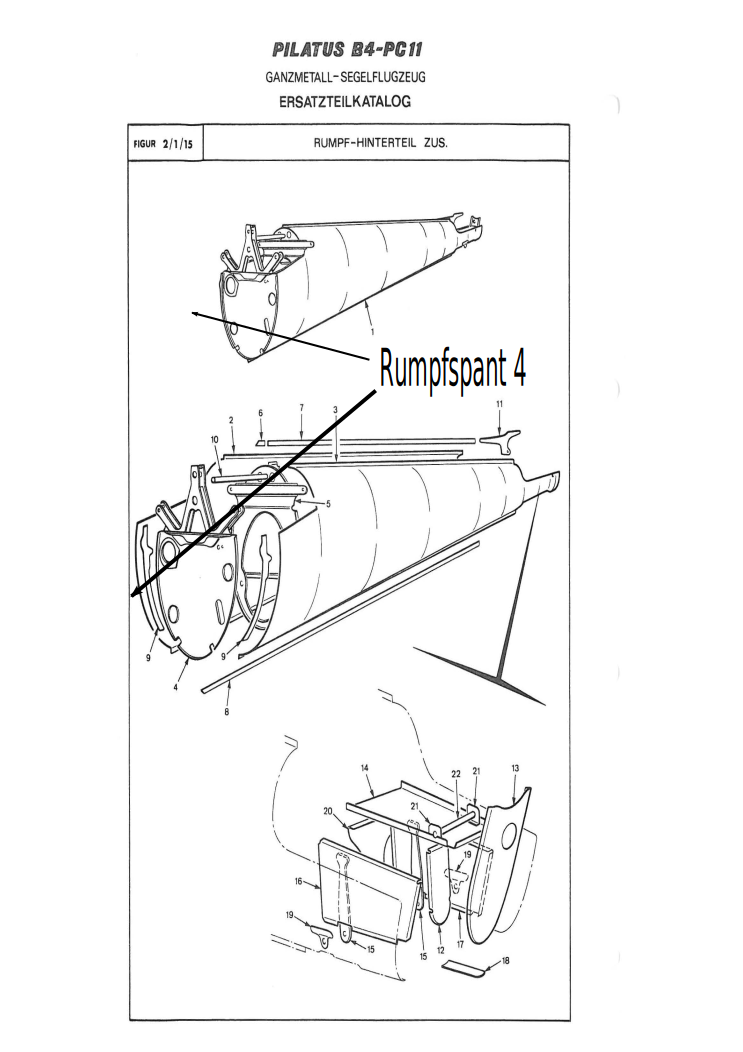
\includegraphics[width=\textwidth,keepaspectratio]{b4_ersatzteil_katalog_fig_2_1_15_annotated}
\caption{Figure 2/1/15 from the Pilatus B4 ersatzteil katalog, with Rumpfspant 4 (referenced in Figure \ref{fig:antenna_location}) pointed out.}
\label{fig:ersatzteil_rumpfspant4}
\end{figure}

\begin{figure}
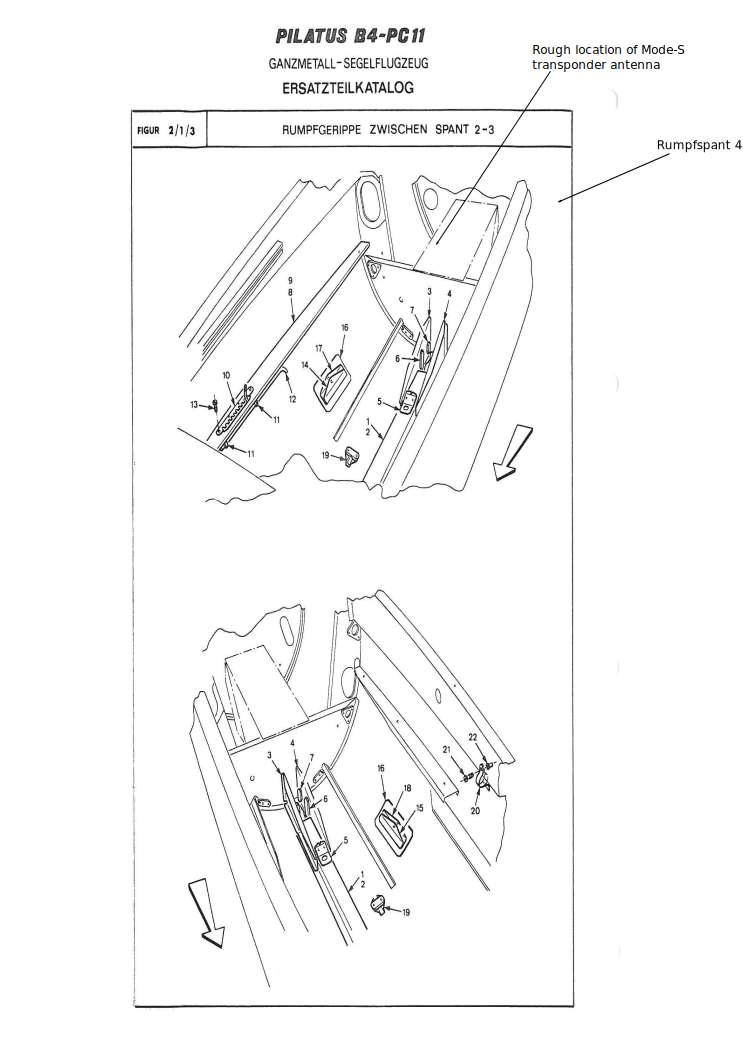
\includegraphics[width=\textwidth,keepaspectratio]{b4_ersatzteil_katalog_fig_2_1_3_annotated}
\caption{Figure 2/1/3 from the Pilatus B4 ersatzteil katalog, with the location of the antenna pointed out.}
\label{fig:ersatzteil_antenna}
\end{figure}

\begin{figure}
\includegraphics[width=\textwidth,keepaspectratio]{outside}
\caption{A photograph, taken from the outside of the fuselage, of the antenna installed.}
\label{fig:outside}
\end{figure}

\begin{figure}
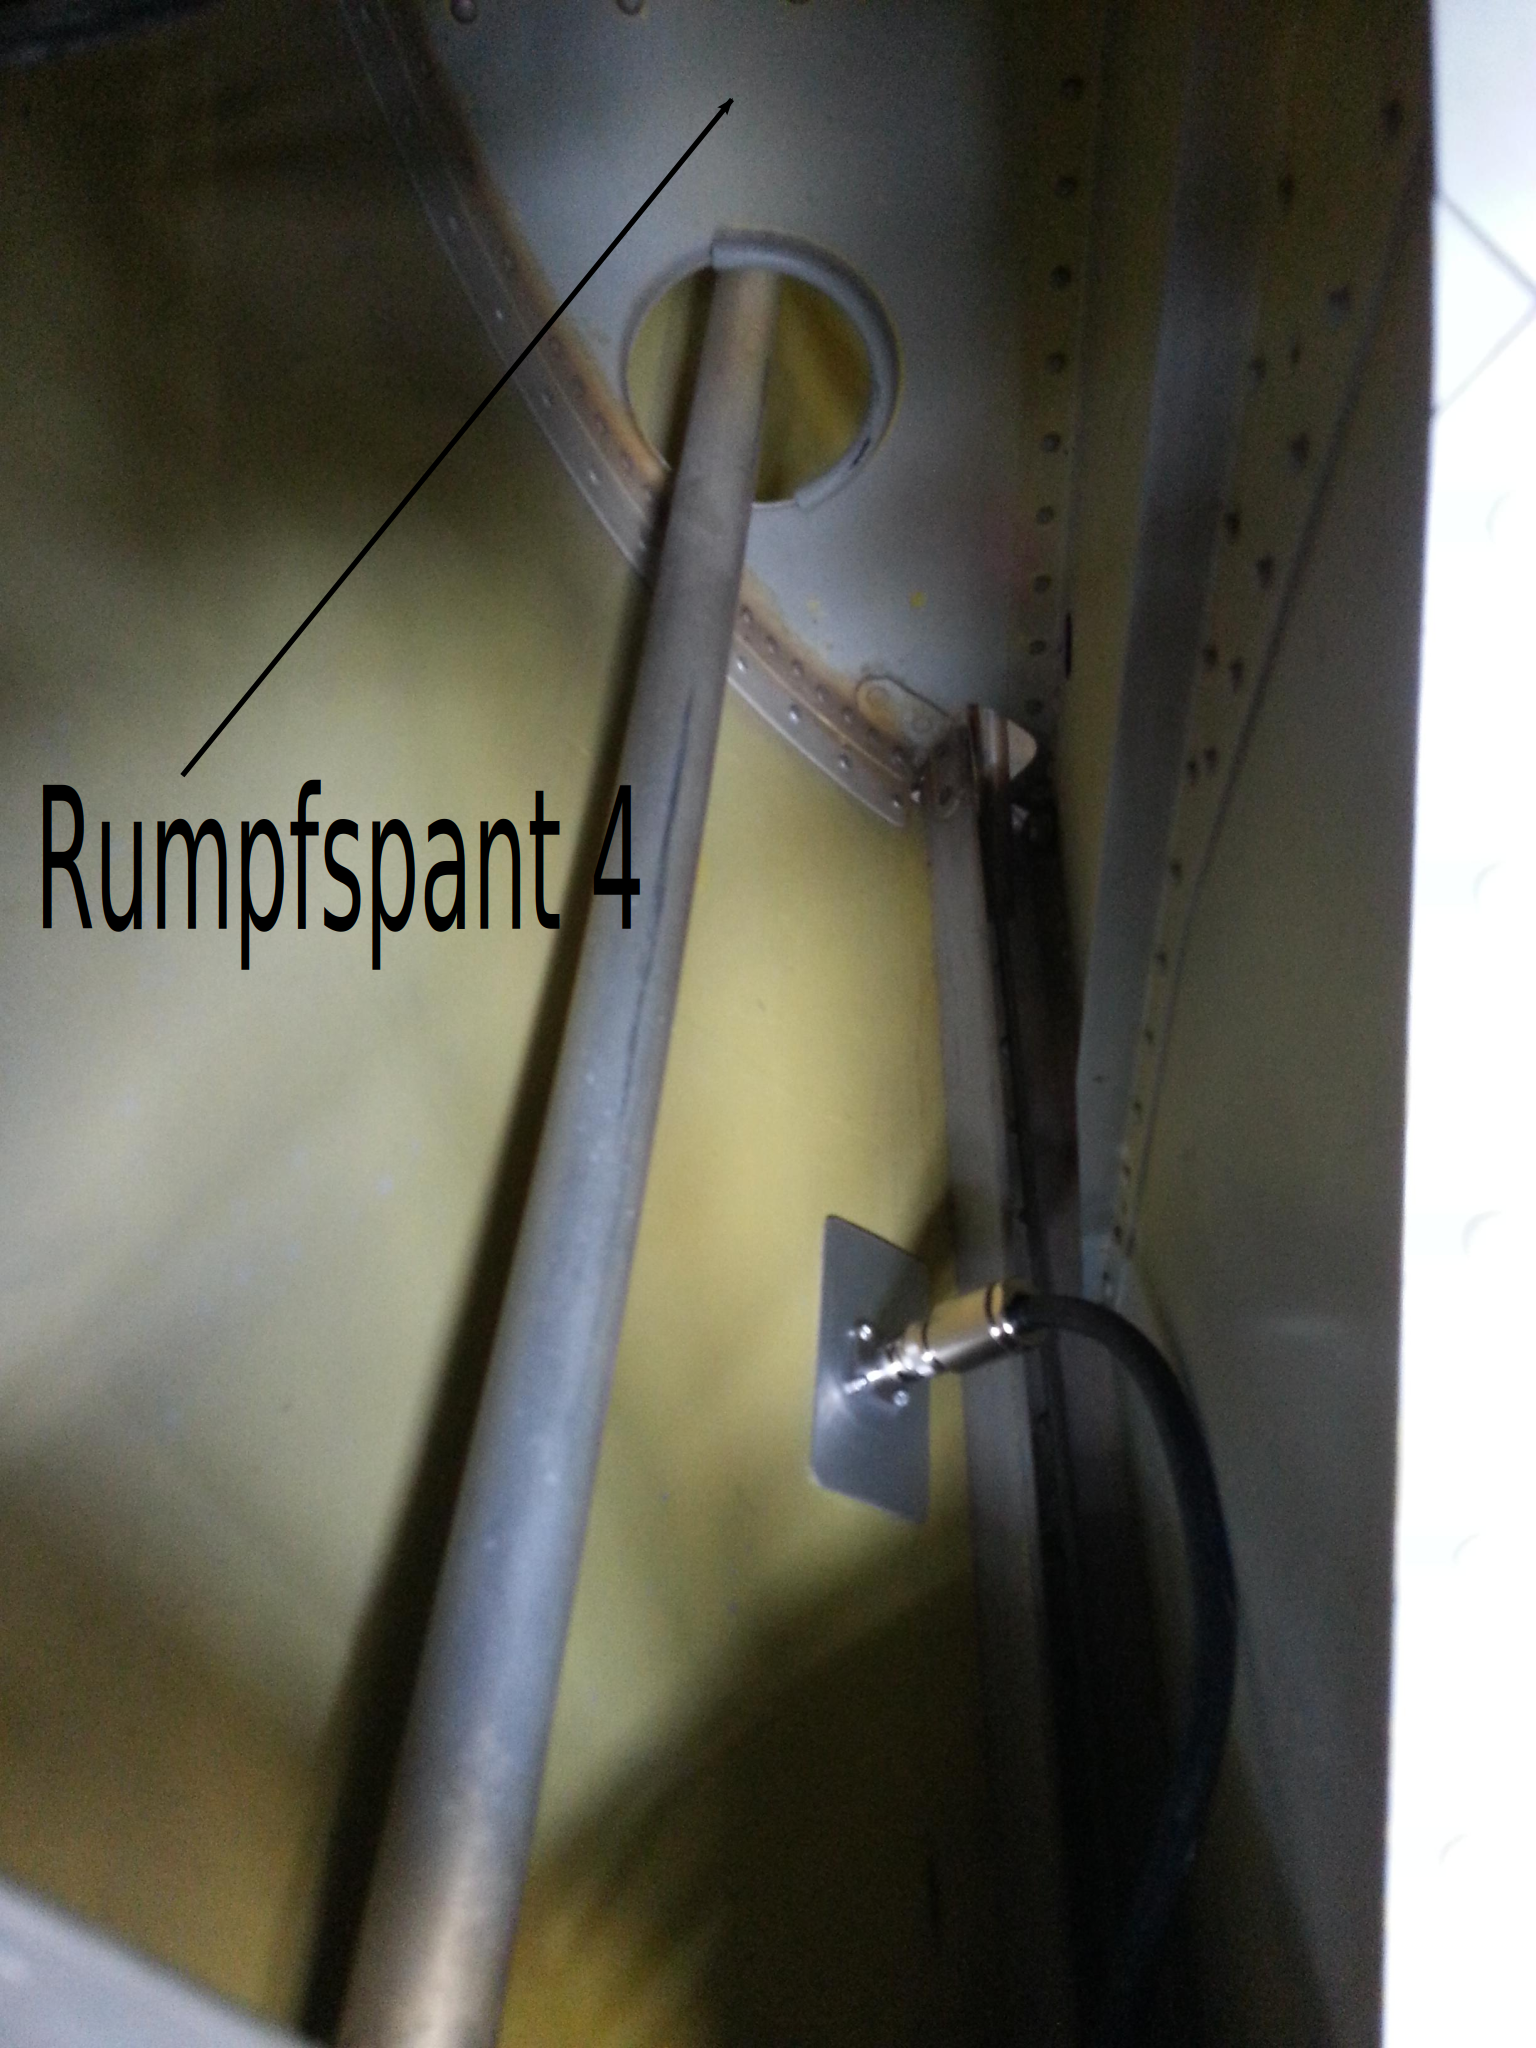
\includegraphics[width=\textwidth,keepaspectratio]{inside}
\caption{A photograph, taken from the inside of the fuselage, of the antenna installed.}
\label{fig:inside}
\end{figure}

\end{document}
